%Orla + Ian 20 dec 04
% 27 Dec: comments of dominic
%TD: update picts

\ifx\wholebook\relax\else
\input{../Common.tex}
\input{../macroes.tex}
\begin{document}
\fi

%%%%%%%%%%%%%%%%%%%%%%%%%%%%%%%%%%%%%%%%%%%
%%%%%%%%%%%%%%%%%%%%%%%%%%%%%%%%%%%%%%%%%%%
\chapter{A First Script and its Implications}\label{cha:firstscript}

While sending messages using direct interaction with a robot is a fun and powerful way of programming robots, it is a bit of a limited way to write more complex programs. Therefore you shall learn the notion of \emph{script}, \ie a sequence of expressions and all the necessary concepts that you will use in this book. Hence, this chapter settles down the vocabulary for the rest of the book. It also serves as a map to the next chapters that will introduce in depth the concepts briefly presented in this chapter.
 
First I present how you to send multiple messages to the same robot separating messages with a semi colon. Then you shall learn how to write script using a dedicated tool called a \index{workspace} workspace. I will describe the different elements that compose a script and  present the possible mistakes that can happen when writing programs.
 
%%%%%%%%%%%%%%%%%%%%%%%%%%%%%%%%%%%%%%%%%%%
\section{Using a Cascade to Send Multiple Messages}
Start to draw a rectangle of 200 height on 100 width. To do so you will start to type the first message \ct{go: 100} hit the return key then click on the robot and type the second expression \ct{turnLeft: 90} and hit the return key, then click on the robot and type the expression \ct{go: 200}... As you quickly notice it this is really tedious. What would be much more handy would be to be able to type everything in one shot and that it gets executed. 

You can send multiple messages to a robot by separating them with  a semi-colon \ct{;}.  To send to a robot  the messages \ct{go: 100}, \ct{turnLeft: 90}, and \ct{go: 200}  simply separate them with a semi-colon \ct{;} as follows \ct{go: 100 ; turnLeft: 90 ; go: 200} (see Figure~\ref{fig:cascading}). This way of sending multiple messages to the same robot is called a \index{cascade}\emph{cascade} of messages in \sq jargon. 

\begin{figure}[!h]
\center{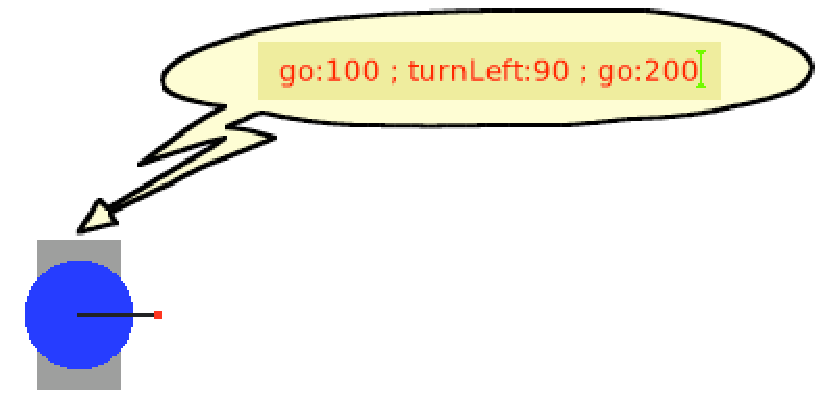
\includegraphics[width=10cm]{goturnleftgo2}}
\center{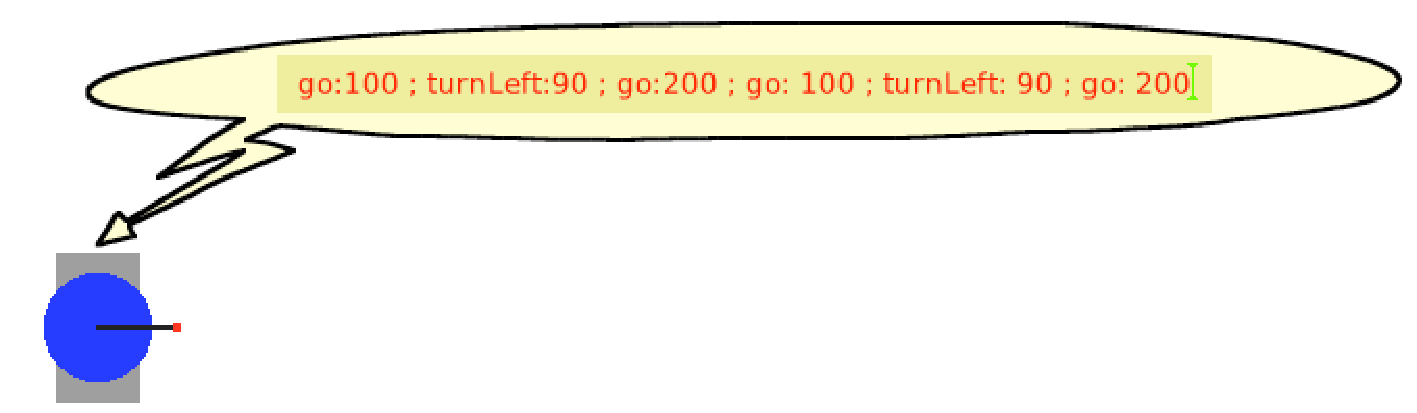
\includegraphics[width=\linewidth]{goturnleftgoLong2}}
\caption{Sending several messages in one shot to a robot using \ct{;}. \label{fig:cascading}}
\end{figure}

However, using a cascade (that is sending multiple messages to a robot separated by the character \ct{;}) does not work well for complex programs. Indeed even for a drawing a simple rectangle is it too long as shown by the second message in Figure~\ref{fig:cascading}. In addition, there are other concerns that professional programmers take into account such as if they can store the sequences of messages and replay them later, whether they can reuse them and not have to type them all the time. For all these reasons, we need other ways to program robots. The first way is to write the sequence of messages, that is called a \emph{script},  in a text editor and ask the environment to execute them as you shall see in a minute. 

\section{A First Script}
The BotInc environment provides a small text editor, called the \tw which is dedicated to script execution (that is executing of the expressions composing a script). Click on the bottom flap called \textbf{Working}, by default it contains a \tw editor as shown by Figure~\ref{fig:TurtleWorkspace}. 

\begin{figure}[!h]
\center{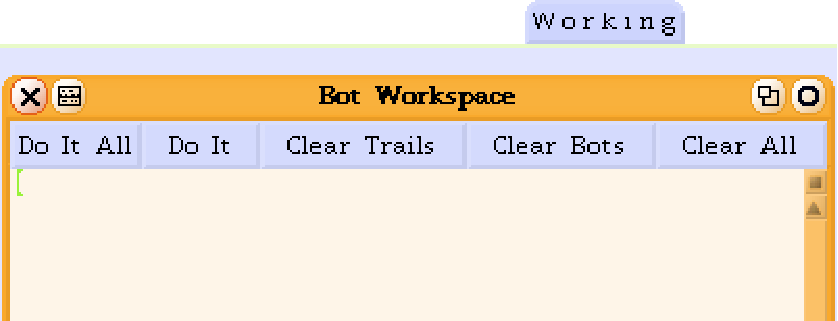
\includegraphics[width=10cm]{TurtleWorkspace}}
\caption{A \tw is a small editor dedicated to the execution of robot scripts. \label{fig:TurtleWorkspace}}
\end{figure}

Let us define a first script  that draws a rectangle and explain it in detail (\scrref{scr:firstScript}).  Figure~\ref{fig:doit} shows the script in a \tw and the result of its execution  obtained by pressing the \button{Do It All} button. Try to get the same result: type the script and press the \button{Do It All} button. Note that I use \ct{pica} as a nickname of picasso since our robots are drawing pictures. 


\begin{scriptwithouttitle}\label{scr:firstScript}
| pica |
pica := Bot new.
pica go: 100.
pica turnLeft: 90.
pica go: 200.
pica turnLeft: 90.
pica go: 100.
pica turnLeft: 90.
pica go: 200.
pica turnLeft: 90
\end{scriptwithouttitle}


The \button{Do It All} button of \tw executes \emph{all} the messages it contains, therefore before typing a script make sure that no other text is already present in the \tw.  Moreover, computers and programming languages cannot deal with even the most obvious mistakes, so be careful to type the text exactly as it is presented in \scrref{scr:firstScript}. Pay attention to type the  \index{class name} uppercase "B" of \ct{Bot} on the second line and to end  each line with \index{dot}\index{period}\index{message separator} a \period. There is no need to put a \period at the end of the last line because there is no other messages to send to the robot.


\begin{figure}[!h]
\center{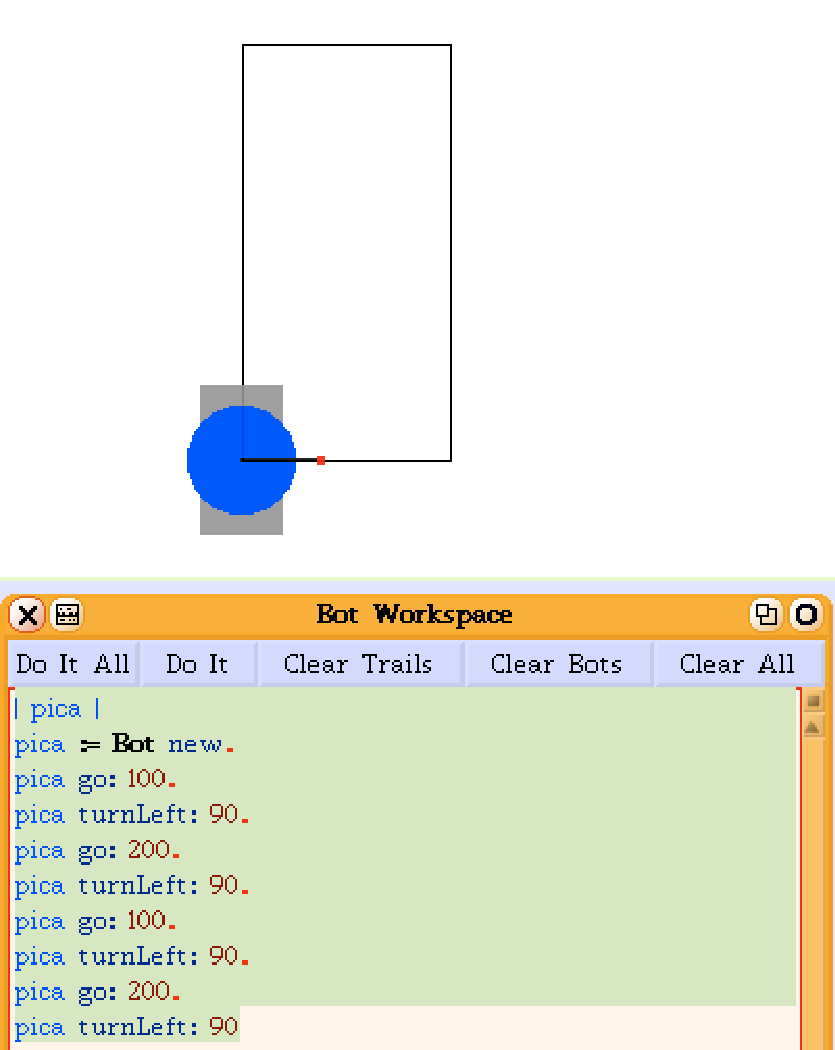
\includegraphics[width=10cm]{fsdoit}}
\caption{A script executed using the \button{Do It All} button of the \tw and its result.\label{fig:doit}}
\end{figure}






\section{\sq and \st}
As you see the script you typed is simple but still it constitutes a program. A program is a list of expressions that a computer can execute. To define programs we need programming languages, \ie languages that allow programmers to define programs that a computer can understand and execute.

\subsection*{Programming Languages}
The idea behind a programming language is to support programmers to express
 solutions to their problems. Support means various things like ease of expression
of the task, efficient execution of the program, reliability of the
resulting application, proof that the program is correct, readibility
of the code written, ease to change the application later on \ldots  There
is no \emph{per se} best language that satisfies all these properties. Programming
languages exhibit different expressive power and properties.

In this book you shall learn how to program in the \st programming language in the \sq environment. \st is a object-oriented programming language like Java or C++. 

\subsection*{\st and \sq}
\sq \index{Squeak} is the name of a \index{programming environment} programming environment. A programming environment is a set of tools that programmers use to
develop applications. \sq contains a lot of tools: text editors,
code browsers, a debugger, an object inspector, a compiler, widgets.... Moreover, \sq contains a lot more for example, you can program music, animate flash files, access the networks, display 3D objects...and much more! However before you can start programming complex applications you have to learn some basic principles and this is the purpose of this book.

\sq programmers develop their applications by writing programs using the
programming language called \index{Smalltalk}\st. \st  is an \emph{object-oriented} language.  This means that objects are created --- virtual objects within the computer, of course --- and these objects are able to understand \index{message} messages that they execute when they receive them. However in the context of this book we will not show you how to define new classes, you will only define new behavior for your robot because object-oriented programming is a bit complex and you have to learn basic programming concepts first.

We chose \st because it is simple, uniform and pure: in \st everything is an object that send messages to other objects and receive messages. In \st there are simple rules and they are always applied consistently. In addition, \st was originally designed for teaching novices how to program. Note that even if \st was designed for novice programmers in mind, large and complex applications have been written in Smalltalk such as the applications controlling the machines that produce the AMD micro-processors that you may have on your current computer. 

Finally, a really interesting aspect of \sq is that it completely written in \st. This implies that if you understand \st you can change, adapt the system to your own needs or 
learn from the system. With \st you have a lot of power in your hands. I hope that you get motivated to learn how to program, but watch out programming like playing piano or painting is not simple, therefore do not be discouraged if you get some difficulties, this is normal and I designed this book so that topics get introduced one after the others smoothly.

\section{Programs, Expressions and Messages}
Now we are ready to take a closer look at your first script and explain it. 
 
\subsection{Typing and Executing Programs}
Let us start by looking at the way you wrote your first script or program (\scrref{scr:firstScript}). You typed a text, a sequence of \emph{expressions}, then you asked \sq to execute it by pressing the \button{Do it All} button. \sq executed the sequence of expressions, that is, it transformed the textual representation of your program into a form that is understandable by a computer, then each expression was performed one after the other. In the first script, the execution created a robot and the robot executed one after the other the messages that were sent to it. 

A program consists of a sequence of \textit{expressions} that are executed by the \sq environment. In this book, we call such a sequence a \index{script} \emph{script}.
  
\largecadre{Vocabulary Point. We called a \emph{script} a sequence of expressions.} 
  
A program is a bit like a cooking recipe. A recipe describes all the steps to cook a meal. A program describes all the steps to produce a certain effect. For example to cook pancakes, the expressions are all the steps we should do to prepare them: mix flavor and milk, add the eggs, heat the pan, etc...

\subsection{Anatomy of a Script}
Now comes the time to understand your first drawing script that I copy here (\scrref{scr:firstScript2}):

\begin{scriptwithouttitle}\label{scr:firstScript2}
| pica |
pica := Bot new.
pica go: 100.
pica turnLeft: 90.
pica go: 200.
pica turnLeft: 90.
pica go: 100.
pica turnLeft: 90.
pica go: 200.
pica turnLeft: 90
\end{scriptwithouttitle}


In a nutshell, the script~\ref{scr:firstScript2} declares that it uses a variable named \ct{pica}  to refer to the robot it creates. Once the robot is created and associated with the variable \ct{pica} the script asks the robot to move to different locations on the screen.  Now let us analyze each line step by step even if certain concepts such as variables will be treated in separate chapters.
  
\begin{description}
\item[\ct{| pica |}] This first line declares a variable. It tells \sq that we want to use the name pica to refer to an object.  Think of it as saying to a friend, from now on I will use the word pica in my sentences\index{variable definition}\index{bar@\texttt{"|}|see{vertical bar}} to refer to a robot. You shall learn more on variables in Chapter~\ref{ch:variables}.

\item[\ct{pica\ :=\ Bot\ new.}] This line creates a new robot by sending the message \ct{new} to the robot class named \ct{Bot} and  associates it with the name \ct{pica}, the variable that we declared before. The word \ct{Bot} requires an uppercase letter \ct{B} because it is a class, that is a factory of robots\index{robot creation}\index{instance creation}.
    
\item[\ct{pica go: 100.}]  The message \ct{go: 100} is sent to the robot we named \ct{pica}. This line can be understood as follows: "pica, move by 100 units of length on the screen". Note that  any message name that terminates by a colon indicates that this message needs additional information, such as a length or an angle. For example, \ct{go: 100} says that the robot should move 100 pixels. The message name is \ct{go:}.

\item[\ct{pica turnLeft: 90.}] This line asks pica to turn 90 degrees  on its left. This lines is again a message sent to the robot named pica.
  
\item The other lines are just repetitions of the previous ones, 
so they have the same effect.
\end{description}




\largecadre{Any \textbf{message} name that terminates by a colon indicates that this message needs additional information, such as a length or an angle. 
\\ \\
For example, the message name \ct{turnLeft:} requires a number representing the angle from which the robot should turn.}

\paragraph{About Pixels.} On a computer screen the unit of distance is called a
\index{pixel}\strong{pixel}. A pixel is the size of the smallest
point which can be drawn on a computer screen. Depending on the type
of computer you are using the actual size of a pixel can vary. You can
see pixels by looking at the screen through a magnifying glass.




%%%%%%%%%%%%%%%%%%%%%%%%%%%%%%%%%%%%%%%%%%%
\subsection{Expressions, Messages and Methods}
Now I should clarify some vocabulary points.

\paragraph{Expression.}
We call an expression\index{expression} any element of a program. Here are some examples of expressions: 

\begin{itemize}
\item \ct{| pica |} is an expression that declares a variable (see Chapter~\ref{cha:variables}).
\item \ct{pica := Bot new} is an operation, called  assignment,  that associates a value to a variable (see Chapter~\ref{ch:variables}). Here, the newly created robot obtained by sending the message \ct{new} to the class \ct{Bot} is associated to the variable \ct{pica}.
\item \ct{pica go: 100} is a message send. The message \ct{go: 100} is sent to  \ct{pica}.
\item \ct{100 + 200} is a message send. The message \ct{+ 200} is sent to  \ct{200}.

\end{itemize}




\begin{figure}[h]
\begin{center}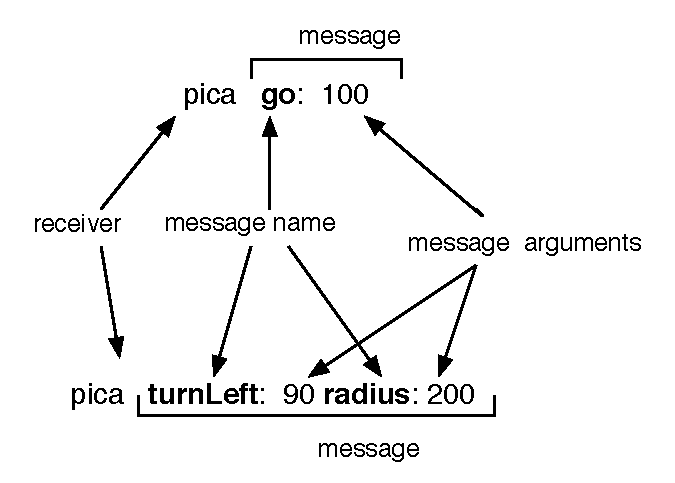
\includegraphics{message}
\caption{Two messages composed of  a message name or method selector, and a set of arguments.\label{fig:firstScriptMessage}}\end{center}
\end{figure}

\paragraph{Message.}
We call a \index{message}\strong{message}, a pair composed of a \strong{message name}\index{selector} also called a \strong{message selector}, and \strong{message arguments}, the required values to execute the message  as shown by Figure~\ref{fig:firstScriptMessage}. A message is sent to a \index{receiver}\strong{message receiver}. \\

\noindent
Example of messages are:
\begin{itemize}
\item In \ct{pica beInvisible}, the message \ct{beInvisible} is sent to a receiver, a robot. This message does not require arguments.

\item In \ct{pica go: 100}, the message \ct{go: 100}  is sent to a receiver a robot. It is composed of the method  name \ct{go:}, and an argument the number \ct{100}. Here, \ct{100} represents the length in pixels of which the robot should move.  Note
that the colon is part of the method selector.

\item In \ct{33 between: 30 and: 50}, the message \ct{between: 30 and: 50} is composed of  the method selector \ct{between:and:}, and two arguments \ct{30} and \ct{50}. This method checks whether the receiver, a number, is between two values, here the numbers \ct{30} and \ct{50}.

\item In \ct{4 timesRepeat: [ pica go: 100 ]}, the message \ct{timesRepeat: [ pica go: 100 ]} sent to the number 4, is composed of  the method selector \timesRepeat, and the argument \ct{[ pica go: 100 ]} a block, a sequence of messages (see Chapter~\ref{ch:looping}).

\item In \ct{100 + 200}, the message \ct{+ 200} is composed of the method selector \ct{+}, and an argument, the number \ct{200}. The receiver is the number \ct{100}.
\end{itemize}



\paragraph{Message separation.}
You have noticed that each line of the script~\ref{scr:firstScript}, except the first one, is terminated by a \period. As we have said earlier, the first line is not a message. Such a line is called a \index{variable declaration} variable declaration in computer jargon. Thus, we can make the following observation: each message must be separated from the following one by a \period. Note that putting a \period after the last message is possible but not mandatory: \st accepts both.

\largecadre{Messages should be separated by a \period. The last statement does not require a terminal \period.

\begin{nalltt}
pica := Bot new.\\
pica go: 100.\\
pica turnLeft: 90.\\
pica go: 100
\end{nalltt}}

\paragraph{Hints.} A \period \ct{.} is a \index{message separation} message \textit{separator} so there is no need to put one if there is no message after it like at the end of a script or a sequence of messages.


\paragraph{Method.}
When  a robot receives a message it executes a \emph{method}\index{method} which is kind of script that has a name.  A method is a named sequence of expressions that a receiver executes in response to a message. For example, the method \go makes the receiver going a certain number of pixels in its current direction. This method \go is executed when a robot receives a message whose name is \go. In the future, I will explain to you how to define new methods for your robot but for now we do not need them to start programming.



\subsection{Using the Cascade}
As I mentioned in the first section of this chapter, you can send multiple messages to the same robot by separating them with a semi-colon, called a cascade. 
In a script, we can also use a cascade (\ct{;}) to send multiple messages to the same robot. \scrref{scr:firstScript2} is equivalent to the following one (\scrref{scr:firstScriptsemi}) where all the messages sent to the same robot are separated by a semi-colon. Using cascades is handy  when you want to avoid to type the receiver of the multiple messages. The cascade is interesting because it shortens scripts. However pay attention that you understand clearly that all the messages are sent to the same receiver.

\begin{scriptwithouttitle}\label{scr:firstScriptsemi}
| pica |
pica := Bot new.
pica 
   go: 100 ; turnLeft: 90 ; go: 200 ; turnLeft: 90 ; 
   go: 100 ; turnLeft: 90 ; go: 200 ; turnLeft: 90.
\end{scriptwithouttitle}



\begin{largecadre}{To send multiple messages to a Bot use a semi-colon \ct{;} to separate the messages, following the template: \ct{aBot message1 ; message2}. \\ \\
For example, \ct{pica    go: 100 ; turnLeft: 90 ; go: 200 ; turnLeft: 90}}
\end{largecadre}

\subsection{About Robot Creation}

To get a new robot you have to send a message, the message \ct{new} to the \emph{class} \ct{Bot}. Note that this is not new! This follows exactly what you did in the previous chapter where you clicked on the blue and orange box named \ct{Bot} representing the class of the same name and typing \ct{new} in the bubble. In \sq, we \emph{always} send messages to objects, robots or classes to interact with them. There is no difference in treatment, except that class and objects understand different messages. Indeed, an object does not know how to create other objects so sending to a robot the message \ct{new} leads to an error and sending the message \ct{color} or \ct{go:} to a class does not make sense and leads naturally to an error. Still in both cases you are sending messages!

Note that other class may provide other messages to create objects such as the class \ct{Color} which returns the color blue or green in response to the messages \ct{blue} or \ct{green}. Do not worry I will always let you know how to get objects of specific classes. 

\largecadre{To get a new object, send the message \ct{new} to a class. \ct{Bot new} creates a new robot. Other classes may offer different messages to get new objects. For example, \ct{Color blue} asks the class \ct{Color} to create a new  color been blue.}

\section{Possible Errors while Writing Programs}
Computers are capable of making highly complex calculations at incredible speed, but they lack the intelligence to correct small mistakes. This means that each expression given to a computer must be given without mistake. The smallest mistakes --- even a lowercase letter instead of an uppercase one --- are likely to be misunderstood by a computer.  In that case, an error message will appear on the screen. This is likely to occur when you are doing your first experiments. So do not despair and try to understand what went wrong. 


\begin{figure}[ht!]
\begin{center}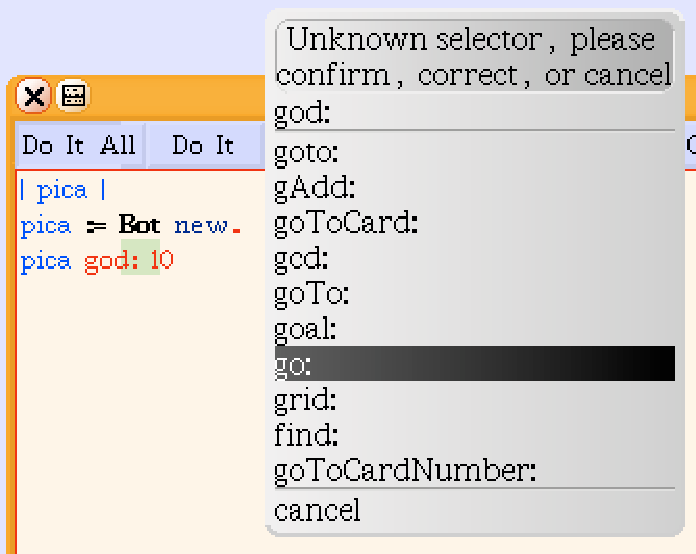
\includegraphics[width=6cm]{errorOne}
\caption{We mispell the message \ct{go:} and type \ct{god:} instead. The message \ct{god:} does not exist therefore \sq prompts us. \label{fig:unknowSelector}}\end{center}
\end{figure}

\sq colors the letters while you are typing, when a word is getting red, this means that you are writing something that \sq does not know. When a word is blue, for a variable or a message, or black for a class, this indicates that everything is correct. In addition, when we execute a message containing an error,  \sq tries to help you by notifying you when it encounters error in the code you wrote.  The error messages that \sq use are in fact menus. The top part in turquoise of the menu window contains a short description of the error; then, depending on the type of error some suggested corrections may be listed as options. Note that you can always cancel  the execution by choosing the cancel choice in the menu and in such a case you must find the place that the computer did not understand, correct it, and retry to execute the script. Here are the most common errors.






\paragraph{Mispelling a message.} You can misspell the name of a message.  In Figure~\ref{fig:unknowSelector} I misspelt the message \ct{go:} and typed \ct{god:} instead.  The message \ct{god:} did not exist therefore \sq turned the word in red. When I tried to execute the script, \sq prompted me. \sq tried to guess what is the message name I wanted to write and it proposed me several messages. I can pick the right message (\ct{go:}) and the message \ct{god:} will be replaced by \ct{go:} or I can simply chose cancel. In that case I will have to change manually \ct{god:} into \ct{go:}.


\begin{figure}[h]
\begin{center}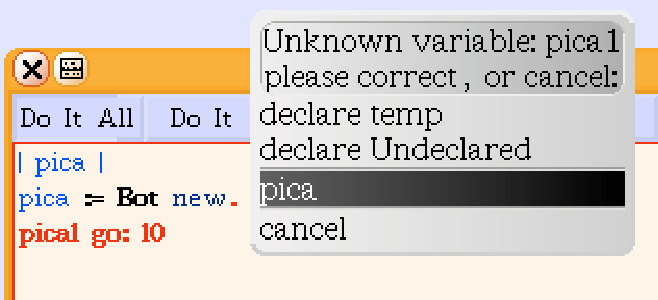
\includegraphics[width=7cm]{mispellVariable}
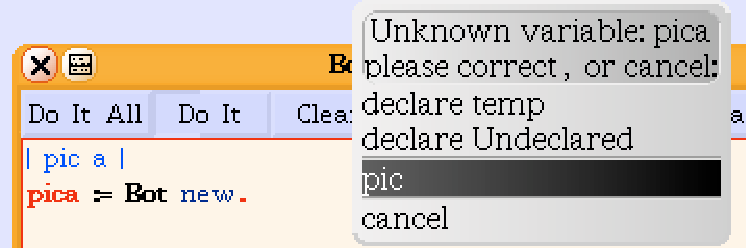
\includegraphics[width=7cm]{unknowVariable}
\caption{Two examples of error. We mistyped the names of the variable. First in the script \ct{pica1} has not been declared and second while defining the variable: \ct{car o} defines two variables \ct{pic} and \ct{a} but not a variable \ct{pica}. \label{fig:wrongVar}}\end{center}
\end{figure} 

\paragraph{Mispelling a variable.} There are two ways to mispell a variable during its declaration (between the two vertical bars \ct{|}) or in the script itself. Figure~\ref{fig:wrongVar} shows the two cases: in the top case I typed \ct{pica1} instead of \ct{pica} in the script. \sq proposed me to define \ct{pica1} as a new variable or to replace \ct{pica1} by \ct{pica}. In the present case choosing \ct{pica} is the solution as shown by Figure~\ref{fig:wrongVar}. The bottom case shows that I misspelt the variable \ct{pica} during its declaration. In fact the space in the middle has for effect to define two variables \ct{pic} and \ct{a}. \sq saw that \ct{pica} was not declared and then it proposed me to declare a new variable with this name or to use the variable \ct{pic}.


\paragraph{Unused variables.} It may happen that we declare too many variables. Even if this is not an error, \ie the program can still run correctly. \sq checks this for us and proposes that we remove the unused variables. For example, in Figure~\ref{fig:unusedVariables} the script only uses the variable \ct{pica} and not \ct{pic} and \ct{a}. Therefore \sq prompts us to remove those. 

\begin{figure}[h]
\begin{center}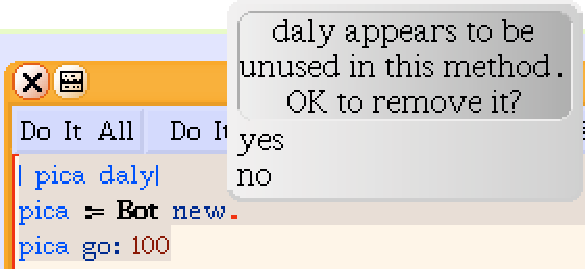
\includegraphics[width=7cm]{unusedVariables}
\caption{All the variables and messages are correct. However the variable \ct{daly} is  defined but not used so \sq indicates it to us. Unused variables are not a problem so you can proceed.\label{fig:unusedVariables}}\end{center}
\end{figure}

\paragraph{Forgetting an uppercase.} Another common mistake is to forget uppercase when needed. Uppercase is needed when you want to send message to object factories. Figure~\ref{fig:TMissing} shows that I typed \ct{bot} instead of \ct{Bot}. \sq tried to find a solution but it fails. In such a case you have to correct it yourself. In the context of this book you only have to pay attention to put an uppercase for \ct{Bot} the robot factory, \ct{Color} the factory of colors.


\begin{figure}
\begin{center}\includegraphics[width=7cm]{BMissing}
\caption{We forgot the uppercase B  to indicate that we want to send a message to the class (the robot factory). We should correct it. \label{fig:TMissing}}\end{center}
\end{figure}


\paragraph{Forgetting a \period.} Finally one of the most common mistakes that even fluent programmers make, is to forget a \period or a cascade between two messages. In such a case \sq thinks that the following variable is just another message and tries to correct it. For example in Figure~\ref{fig:periodMissing} a \period is missing after the expression \ct{pica := Bot new} therefore \sq tries to send the message \ct{pica} and this message does not exist, therefore it tries to propose a replacement but failed to find. In such a case, you have to cancel and type the \period manually.

\begin{figure}[h!]
\begin{center}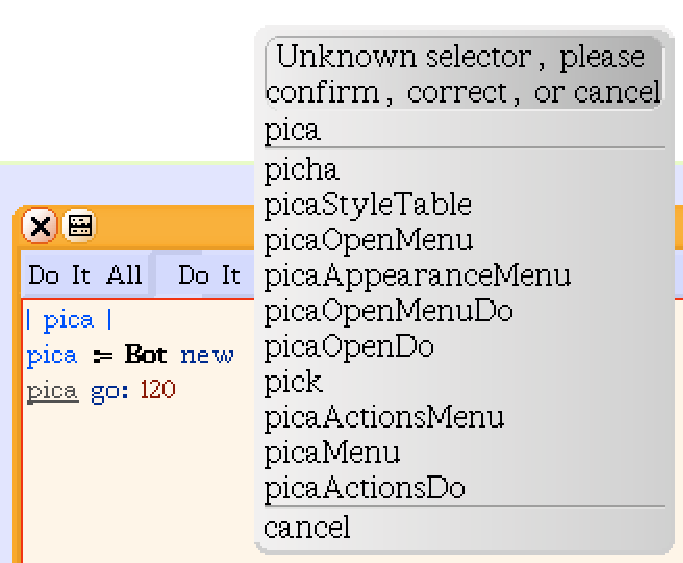
\includegraphics[width=6cm]{periodMissing}
\caption{Two examples of error. We mistyped the names of the variable. First in the script \ct{pica1} has not been declared and second while defining the variable: \ct{car o} defines two variables \ct{car} and \ct{o} but not a variable \ct{pica}. \label{fig:periodMissing}}\end{center}
\end{figure} 

\paragraph{About Colored Words}
\sq tries to identify mistakes when you are typing your scripts and it provides some visual clues on the possible errors. Figure~\ref{fig:coloring} shows some typical situations: 
\begin{itemize}
\item{(a)} I started to type the first letter of an undeclared or unknown variable. As there is no variable starting with the letter x, \sq turned the x in red, letting me know that I was doing a mistake. 
\item{(b)} I finished to typed a variable which is declared, therefore \sq turns it into blue to let me know that the variable is declared. 
\item{(c)} I'm writing a variable whose beginning is the one of a declared variable so \sq underline it to let me that I'm going well. 
\item{(d)} As soon as I type a character that leads to a variable that is not declared, \sq turns it in red. Note the difference with the previous case. In case (c) I could have typed the character a and then completed the word pica as in (a), I typed the character b and ended up with a undeclared variable (\ct{picb}). 
\item{(e)} After having typed the name of a declared variable (as in case (b)), I added an extra character a and this leads to the name of an unknown variable (\ct{picaa}).
\item{(f)} \sq tries to do the same for the message names. Here I misstyped the message \ct{go:} and typed instead \ct{gou}. As soon as I typed the character u, \sq saw that the message name \ct{gou} was unknown so it turned it in red. 
\item{(g)} \sq tries to  do the same for the classes. Here I typed the character w after Bot and \sq indicates to me that there is no class named \ct{Botw} in the system.
\end{itemize}


\begin{figure}[h!]
\begin{center}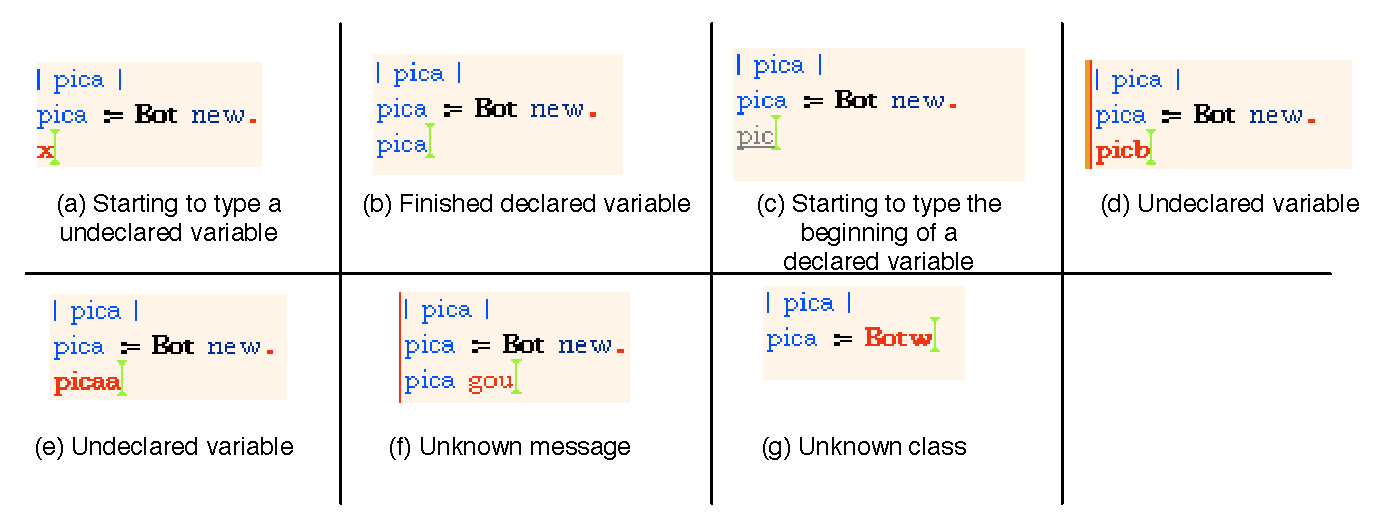
\includegraphics[width=12cm]{coloring}
\caption{\sq using colors to help finding mistakes. \label{fig:coloring}}\end{center}
\end{figure} 




\summa
\begin{itemize}
\item \emph{To execute an expression}. Press the \button{Do It All} button of the workspace.




\item A \emph{script} is a sequence of expressions that perform a task.

\item A message is composed of a message name, and some arguments. Some message may not required arguments. For example \ct{pica beInvisible} 

\item Any message name terminated by a colon indicates that this message needs additional information, such as a length or an angle for example. For example, the message name \ct{turnLeft:} requires a number representing the angle from which the robot should turn.

\item To get a new object, send the message \ct{new} to a class. \ct{Bot new} creates a new robot. Other classes  may offer different messages to get new objects. For example, \ct{Color blue} asks the class \ct{Color} to create a new  color been blue.


\item A class is a factory of objects. Class names always start with an uppercase letter. Here \ct{Bot} is the factory creating new robots and \ct{Color} the one creating colors. \

\begin{nalltt}
Bot new color: Color blue
\end{nalltt}

\item Messages should be separated by a \period. Terminal \period is not required.\

\begin{nalltt}
pica := Bot new.
pica go: 100.
pica turnLeft: 90.
pica go: 100
\end{nalltt}


\item To send multiple messages to the same object use a semi-colon \ct{;} to separate the messages, following the template: \ct{aBot message1 ; message2}. For example, \ct{pica    go: 100 ; turnLeft: 90 ; go: 200 ; turnLeft: 90} send the message \ct{go: 100}, \ct{turnLeft: 90}, \ct{go: 200}, \ct{turnLeft: 90} to the same robot named \ct{pica}.
\end{itemize}







\ifx\wholebook\relax\else
\end{document}\fi







\ifx\wholebook\relax\else\end{document}\fi



